\documentclass[11pt]{article}
\usepackage[margin=1in]{geometry}
\usepackage[T1]{fontenc}
\usepackage{amsmath,amssymb,booktabs,graphicx,hyperref,xcolor,array,caption,colortbl,multirow}
\usepackage[numbers,sort&compress]{natbib}
\newcommand{\todo}[1]{{\color{red}[\textbf{TODO:} #1]}}
\newcommand{\cn}[1]{{\color{orange}[\textbf{CITATION NEEDED:} #1]}}
\newcommand{\verify}[1]{{\color{blue}[\textbf{VERIFY:} #1]}}
\newcommand{\best}[1]{\cellcolor{gray!18}#1}

\title{How Far Can Simulation Take Root Cause Diagnosis in Milling?\\
Provenance-Tracked Simulation, Real-Data Gap Measurement and the Circularity of Simulated RCA Benchmarks}
\author{\textit{Author names and affiliations to be added}}
\date{\textbf{DRAFT v2} --- target venue not yet chosen; real multi-cause data not yet collected (Section~\ref{sec:limits})}

\begin{document}
\maketitle

\begin{abstract}
Diagnosing the root cause of a machining fault (loose fixture, worn tool, excessive depth, unsuitable spindle speed) is attractive to train on simulated data, because real cuts with known causes are scarce.
Whether simulation actually supports such diagnosis is rarely measured: simulated benchmarks usually build the diagnostic nodes from the same generator that produces the test faults, and the gap to real signals is not quantified component by component.
We therefore treat simulation-based diagnosis as a measurement problem.
We build a regenerative-milling simulator in which every parameter is tagged as fixed, ranged, learned or assumed, ground its healthy baseline in real multi-sensor spectra, and compare it with real data along three axes: healthy baseline, fault signature, and transfer to unseen machines.
In a causal root-cause-ranking benchmark, top-1 accuracy at ten anomalous samples is 0.80--0.98 for five of six algorithms when nodes and faults share a generator, but 0.35--0.71 when the generator's physical parameters are shifted at test time; replacing the causal graph by a shuffled or empty one changes nothing, and label-free nodes give near-chance accuracy, so the benchmark measures supervised node estimation, not causal reasoning.
The simulated healthy baseline remains distinguishable from real data (balanced accuracy $0.82\pm0.04$), and neither the simulated faults nor a once-per-revolution chipped-flute mechanism reproduces the low-frequency, tonal signature of a real defective tool.
On a public three-machine wear dataset, a model trained only on simulated wear and applied to unseen machines without real labels reaches wear-detection AUROC 0.89, 0.81 and 0.57, which is below a one-feature force-RMS rule on two of the three machines (0.99, 0.99, 0.46), and fine-tuning it with real labels is no better than training from scratch (at earlier-wear thresholds it is higher than the rule on average, but only because of one machine); domain-adaptation baselines add nothing over gradient boosting on this task.
Transfer to unseen machine--tool combinations does not degrade with a spectral proxy for dynamics distance (nine targets), so these data cannot test whether simulation is needed to extrapolate to new dynamics.
We conclude that this wear task is too easy to show a benefit of simulation, that benchmark design can inflate apparent diagnostic accuracy, and we release the protocol to test these conclusions on harder, real multi-cause data.
\end{abstract}

%% ---------------------------------------------------------------------------------------------
\section{Introduction}
Machine-tool operators and process engineers need to know \emph{why} a milling operation misbehaves, not only \emph{that} it does, because the remedy differs: re-clamp the part, change the tool, reduce the depth or move the spindle speed.
Public machining datasets record sensor streams and, at best, expert labels of normal or abnormal operation; ground-truth root causes are rare \citep{kim2026msm}.
Simulation is the obvious substitute, and training on simulated data and applying it to a real machine has been shown to work for chatter detection \citep{alberts2024sim2real} and tool-fault monitoring \citep{ebrahimi2023smartfaults}.
Both studies, however, consider a single fault family on one machine, and neither asks how much of the reported accuracy comes from the simulator itself.

\paragraph{The unresolved problem.}
For root cause analysis, the gap between a simulated benchmark and real diagnosis has three separate parts that existing work does not separate: (i) the healthy baseline of the simulator may differ from real signals; (ii) the simulated fault signatures may differ from real ones; and (iii) the diagnostic procedure may exploit the generator, for example when the nodes of a causal graph are trained on labels produced by the same simulator that generates the test faults.
Without separating them, a high simulated accuracy cannot be interpreted.

\paragraph{Our approach.}
We build a simulator whose parameters carry their provenance and measure each part of the gap against real data (Figure~\ref{fig:pipeline}).
The healthy baseline is modelled from real spectra rather than simulated, so that part (i) can be tested directly; fault signatures are compared with a real defective tool for part (ii); and part (iii) is tested by shifting the generator's parameters at test time and by ablating the graph and the node construction.

\paragraph{Contributions.}
\begin{enumerate}
\item \textbf{A measurement of benchmark circularity.} We show that top-1 accuracy of six causal RCA algorithms falls from 0.80--0.98 to 0.35--0.71 under moderate parameter shift, that the causal graph carries no information in the benchmark, and that the result is decided by how nodes are constructed (Section~\ref{sec:circ}).
\item \textbf{A component-wise gap measurement with negative results.} A real-data baseline and a classifier two-sample test quantify the healthy gap; a real defective tool shows that low-frequency and tonal components are not reproduced by any simulated fault, including a chipped-flute mechanism (Sections~\ref{sec:healthy} and~\ref{sec:real}).
\item \textbf{Evidence on when simulation helps on real data.} On a public multi-machine wear dataset, simulation-only transfer is machine-dependent and below a one-feature baseline, fine-tuning gives no benefit, and domain-adaptation baselines add nothing, so the task cannot show a benefit of simulation (Section~\ref{sec:wear}).
\item \textbf{A parameter-provenance policy, a simulator with FRF import, and an evaluation protocol} to be run on real multi-cause data when available (Sections~\ref{sec:method} and~\ref{sec:limits}).
\end{enumerate}

\paragraph{What we do not show.}
We have no validation of root-cause \emph{ranking} on real multi-cause data. Simulation remains the only practical source of labelled data for causes that cannot be collected in numbers, so we do not argue that it is unnecessary; we show that its fidelity is not yet established and that, on the real data we could test, it was not needed. Whether it is needed for causes without real labels, or for machines outside the training dynamics, is the question the protocol of Section~\ref{sec:limits} is designed to answer.

\begin{figure}[t]\centering
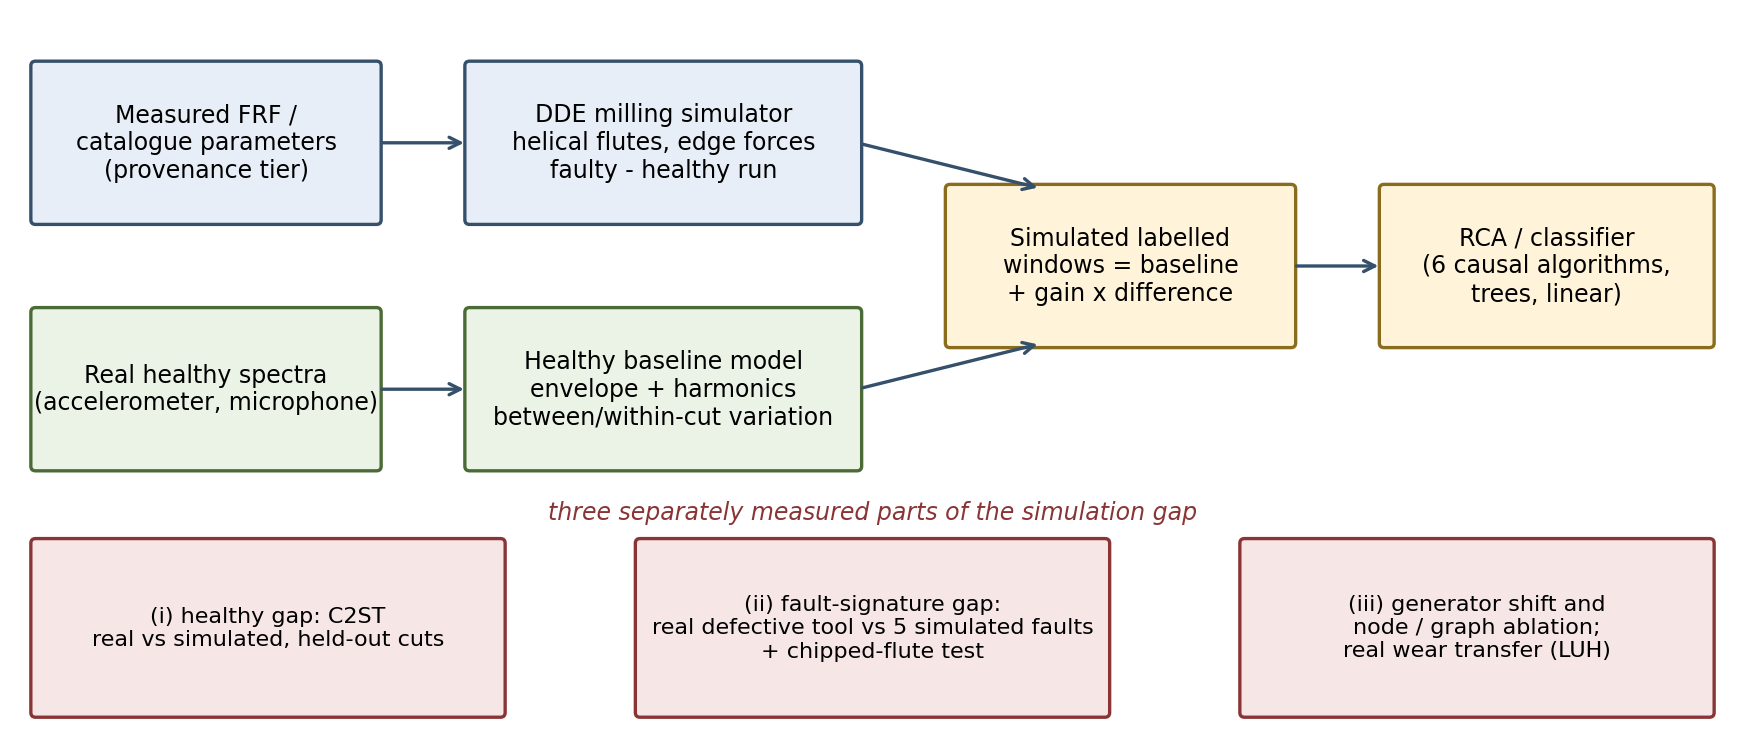
\includegraphics[width=0.97\linewidth]{figures/pipeline.png}
\caption{Overview of the study: the simulator supplies fault differences only, the healthy baseline comes from real data, and each part of the sim--real gap is tested separately.}\label{fig:pipeline}
\end{figure}

%% ---------------------------------------------------------------------------------------------
\section{Related Work}
\paragraph{Simulation-trained diagnosis in machining.}
\citet{alberts2024sim2real} train a random forest on more than 140\,000 simulated chatter cases, then fine-tune it with 10\% of 1\,600 real instances from one custom 3-axis machine to reach 86.1\% accuracy on a chatter-versus-stable decision.
\citet{ebrahimi2023smartfaults} train on process simulations to monitor tool-related faults \verify{read full text before quoting numbers}, and \citet{yesilli2022tlchatter} transfer chatter detectors between conditions.
These works establish that simulation-to-real training is feasible for one fault family on one machine; they do not address several root causes, a change of machine, or the share of accuracy attributable to the generator.

\paragraph{Transfer across machines and conditions for tool wear.}
Domain-adversarial transfer \citep{wang2020datwear}, meta domain generalisation \citep{li2023metadg} and physics-guided or hybrid models \citep{li2025physguided,yang2022hybridwear} address changes of cutting condition or machine for wear, using real data of the source domains. We use these as the reference class of baselines for future real data (Section~\ref{sec:limits}), but not as baselines here, since no real multi-cause data are available.

\paragraph{Causal root cause analysis.}
RCD \citep{ikram2022rcd} localises root causes with conditional-independence tests, BARO \citep{pham2024baro} uses Bayesian change-point detection, and \citet{orchard2025} study outlier root causes without full structural knowledge. These were developed for software systems; applying them to machining needs a data source with known causes, which is the role of simulation here. BRCD, RCG and SimpleRCA are implemented from their repository descriptions \cn{bibliographic entries for BRCD (ICML 2026), RCG (UAI 2025), SimpleRCA (2025) to be added; the author confirms the sources}.

\paragraph{Calibrating simulators to data.}
Calibration with a discrepancy term \citep{kennedy2001}, domain randomisation \citep{tobin2017}, adversarial refinement \citep{shrivastava2017} and simulation-based inference \citep{cranmer2020} are the standard tools. We use a classifier two-sample test as a diagnostic, not as a training signal \cn{Lopez-Paz and Oquab 2017}.

%% ---------------------------------------------------------------------------------------------
\section{Study Design and Data}\label{sec:data}
We use three real sources, each for one question (Table~\ref{tab:data}).
\begin{table}[t]\centering\small
\caption{Real data used and the question each answers.}\label{tab:data}
\begin{tabular}{p{3.2cm}p{5.8cm}p{5.2cm}}\toprule
Source & Content used & Question\\\midrule
MSM, machine \texttt{imi\_vm20i}, datasets 5, 6 \citep{kim2026msm} & 73 cuts (48 normal, 25 abnormal), 2-flute 6.35~mm tool, AA~6061, 9000--12000~rpm, three radial depths, 219 windows of 0.3~s & Healthy baseline and gain calibration (Sec.~\ref{sec:healthy})\\
MSM datasets 3 and 14 & Intentionally defective 12.7~mm four-flute tool D$^*$ (12 cuts) and healthy tool (64 cuts), AISI 4140 & Fault signature (Sec.~\ref{sec:real})\\
LUH \citep{denkena2023luh} & Three machines $\times$ three tools, force at 25~kHz, flank wear VB & Cross-machine transfer and sim-to-real wear (Sec.~\ref{sec:wear})\\\bottomrule
\end{tabular}
\end{table}
In datasets 5 and 6 the abnormal label is strongly associated with up-milling (all 36 down-milling cuts are normal), so it is not a specific root cause. Spindle speed and feed in the label files equal the controller-recorded values (ratio 1.000).

%% ---------------------------------------------------------------------------------------------
\section{Method}\label{sec:method}
\subsection{Overview}
Given a cutting condition, the framework produces labelled simulated windows in three steps: a delay-differential-equation simulator provides the effect of a fault as a \emph{difference} between a faulty and a healthy run (Section~\ref{sec:sim}); a baseline model fitted to real spectra provides the healthy signal (Section~\ref{sec:base}); and the scaled difference is added to the baseline (Section~\ref{sec:fault}). Section~\ref{sec:proto} defines the RCA protocols that consume these windows.

\subsection{Provenance-tracked regenerative simulator}\label{sec:sim}
\paragraph{Motivation.} Simulated parameters that have no source can silently decide a benchmark's outcome, and the context of a literature value (tool, material, operation) is easily lost.
\paragraph{Design.} Tool-tip motion follows modal dynamics driven by cutting force; the chip thickness of each of $N_z{=}8$ axial slices depends on the current and delayed displacement, with helix lag $\psi(z)=2z\tan\beta/D$ and
\begin{equation}
dF_t=(K_t h+K_{te})\,dz,\qquad dF_r=(K_r K_t h+K_{re})\,dz,
\end{equation}
where $h\ge 0$ is the chip thickness, $K_{te},K_{re}$ are edge coefficients and $\beta{=}30^\circ$ (manufacturer series feature list; medium confidence). Spindle imbalance adds a synchronous force $U\Omega^2$, and optional effective runout adds a once-per-revolution term. Each parameter is \emph{fixed} when a verified source gives it for this exact context, a \emph{range} when a source gives one, \emph{learned} when only data constrain it, and \emph{assumed} otherwise (Appendix~\ref{app:registry}). Force coefficients, tool-tip dynamics and imbalance for the simulated tool had no usable source, and our attempts to learn them failed (Section~\ref{sec:neg}); they are nominal values.
\paragraph{Advantage and check.} The tier makes every unsupported assumption visible to a reader. With helix and edge forces off the implementation matches a straight-flute reference to $7\times10^{-16}$, eight axial slices are converged, and a time-domain grid agrees with the zero-order stability-lobe prediction on 79\% of speed--depth points, with disagreement at moderate depth where the zero-order approximation is known to be conservative (Figure~\ref{fig:lobes}).
\begin{figure}[t]\centering
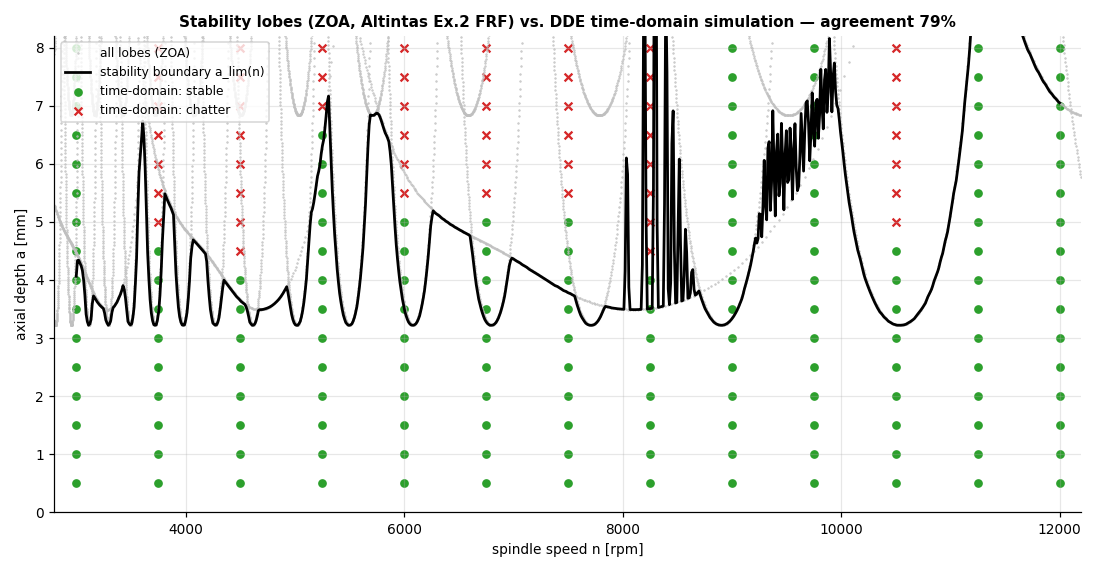
\includegraphics[width=0.78\linewidth]{figures/exp1_lobes_validation.png}
\caption{Stability lobes (zero-order approximation, 4-flute reference transfer function) and time-domain outcomes on a speed--depth grid.}\label{fig:lobes}
\end{figure}

\paragraph{FRF import.} For a new machine the tool-tip transfer function can be read from hammer-test data (receptance, or accelerance divided by $(j\omega)^2$) and fitted by adding modes at residual peaks with linear residue estimation. On synthetic transfer functions with added noise the shape error is 0.8\% (no noise), 1.7\% (noise 1\% of the peak) and 16\% (3\%, one mode lost); it has not been tested on measured FRFs.

\subsection{Healthy baseline from real spectra}\label{sec:base}
\paragraph{Motivation.} Fitting the simulator's absolute signal levels directly to real windows did not converge (Section~\ref{sec:neg}); the data constrain the \emph{healthy signal} far better than the physics constants.
\paragraph{Design.} For each 0.3~s window we compute the power spectral density of two accelerometer channels and the microphone and summarise it by a piecewise-linear envelope over log-frequency (18 knots, band-averaged linear power so that energy is preserved) plus the rms of the first eight harmonics of the spindle frequency. Envelope parameters are regressed on the cutting conditions (kernel ridge on $\log n$, $\log a_e$, $\log f$, direction); out-of-fold residuals are split by one-way variance analysis into between-cut and within-cut parts on twelve principal directions. Windows are synthesised by shaping complex Gaussian spectra with the envelope and adding harmonics with random phases (real spectra in Figure~\ref{fig:psd}).
\paragraph{Advantage.} The healthy part of a simulated window is real-data-driven, so any remaining difference to real data (Section~\ref{sec:healthy}) can be attributed to the baseline model, not to the physics.
\begin{figure}[t]\centering
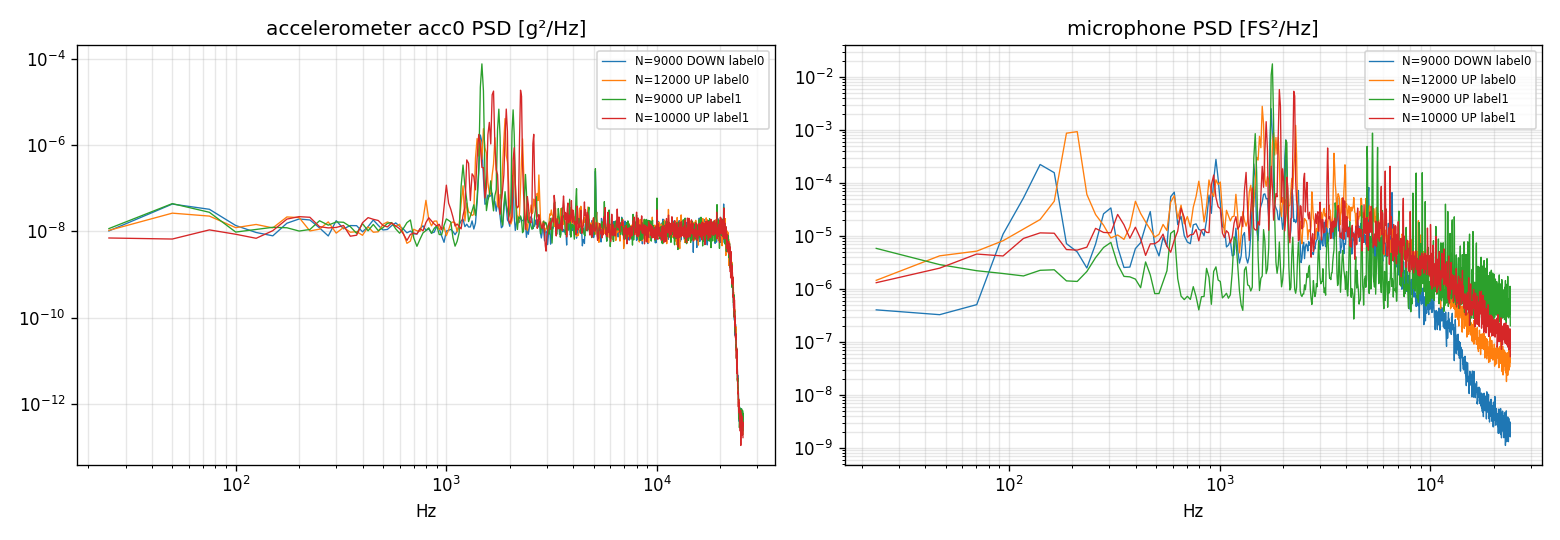
\includegraphics[width=0.95\linewidth]{figures/real_psd_examples.png}
\caption{Power spectral density of four real windows (accelerometer left, microphone right): normal and abnormal cuts at different spindle speeds.}\label{fig:psd}
\end{figure}

\subsection{Fault injection with effect-size gain}\label{sec:fault}
\paragraph{Motivation.} A simulator's absolute fault amplitude is unknown, but the \emph{direction} of a fault's effect on the signal is physically constrained.
\paragraph{Design.} For each window and fault we run the simulator twice with the same condition and noise seed and add $g\,(s_\text{fault}-s_\text{healthy})$ to the baseline, with separate $g_\text{acc},g_\text{mic}$. Faults and ranges (assumed): stiffness $\times[0.4,0.9]$; damping $\times[0.3,0.8]$; tool wear $K_t\times[1.1,1.6]$ with higher edge force; radial depth $\times[1.5,4]$; spindle speed $\pm[3,15]\%$. Matching feature distributions did not identify the gains (flat objective), so we set them by effect size: the mean shift of $\log_{10}$ acceleration rms and microphone level equals the real abnormal--normal difference ($+0.375$ and $+4.86$~dB), giving $g_\text{acc}=7.7\times10^{-6}$ and $g_\text{mic}=0.0116$.
\paragraph{Limit.} Real abnormal windows are mainly up-milling cuts, so the scale is an assumption about fault strength, not an estimate (Section~\ref{sec:sweep}).

\subsection{RCA protocols}\label{sec:proto}
\paragraph{Causal ranking.} Following the root-cause-ranking protocol of the repository, a healthy dataset $D_\text{obs}$ and $m$ anomalous samples $D_\text{int}$ are given and each algorithm ranks 14 nodes: five root-cause nodes (estimated stiffness, damping, wear, depth; controller-measured spindle-speed deviation) and nine sensor nodes (log acceleration, microphone level, two non-synchronous indices, three accelerometer and two microphone bands). The directed graph encodes physical prior knowledge. The first four root-cause nodes are gradient-boosted soft sensors of the log fault factor, trained on training cuts only (out-of-fold for $D_\text{obs}$). Cuts are split by identity (43 training, 30 test; stratified by $a_e$); each point averages 100 random draws of $m$ faulty windows per fault.
\paragraph{Generator shift.} Because the soft sensors are trained on labels from the same generator, a \emph{shifted} test multiplies natural frequency, damping, stiffness, force and edge coefficients by random factors in $[0.75,1.33]$, $[0.5,2]$, $[0.6,1.7]$, $[0.6,1.6]$ and $[0.4,2.5]$ per cut, with soft sensors left at their nominal training.
\paragraph{Real-data transfer protocol.} For real data, features are expressed relative to the healthy baseline of each tool, are invariant to the sign convention of the force axes (absolute mean force), and models are evaluated leave-one-machine-out; training modes are simulation only, simulation then fine-tune on $k$ real samples, and real only.

%% ---------------------------------------------------------------------------------------------
\section{Experiments}
\subsection{Is the benchmark circular? Generator shift and ablations}\label{sec:circ}
\paragraph{Question and protocol.} Does the accuracy of causal RCA algorithms reflect diagnosis, or the match between nodes and generator? We compare shared-generator and shifted settings (Table~\ref{tab:causal}, Figure~\ref{fig:causal}) and ablate graph and node construction (Table~\ref{tab:ablation}; three seeds, each changing the cut split and data; 60 draws per fault).
\begin{table}[t]\centering\small
\caption{Causal RCA: top-1 accuracy (mean over 5 faults; 100 draws per fault; chance $=1/14\approx0.07$) versus number of anomalous samples $m$.}\label{tab:causal}
\begin{tabular}{l cccc cccc}
\toprule
& \multicolumn{4}{c}{Same generator} & \multicolumn{4}{c}{Shifted generator parameters} \\
\cmidrule(lr){2-5}\cmidrule(lr){6-9}
Algorithm & $m{=}5$ & $10$ & $20$ & $50$ & $m{=}5$ & $10$ & $20$ & $50$ \\
\midrule
BRCD & 0.87 & 0.90 & 0.89 & 0.85 & 0.59 & 0.58 & 0.62 & 0.64 \\
RCD & 0.79 & 0.80 & 0.71 & 0.59 & 0.45 & 0.39 & 0.30 & 0.21 \\
RCG & 0.87 & 0.90 & 0.89 & 0.85 & 0.58 & 0.59 & 0.63 & 0.64 \\
Smooth Traversal & \cellcolor{gray!20}\textbf{0.95} & \cellcolor{gray!20}\textbf{0.98} & \cellcolor{gray!20}\textbf{1.00} & \cellcolor{gray!20}\textbf{1.00} & \cellcolor{gray!20}\textbf{0.68} & \cellcolor{gray!20}\textbf{0.71} & \cellcolor{gray!20}\textbf{0.77} & \cellcolor{gray!20}\textbf{0.81} \\
BARO & 0.88 & 0.94 & 0.98 & 1.00 & 0.42 & 0.35 & 0.30 & 0.26 \\
SimpleRCA & 0.53 & 0.52 & 0.52 & 0.48 & 0.42 & 0.44 & 0.44 & 0.40 \\
\midrule
Chance (1/14) & 0.07 & 0.07 & 0.07 & 0.07 & 0.07 & 0.07 & 0.07 & 0.07 \\
\bottomrule
\end{tabular}

\end{table}
\begin{figure}[t]\centering
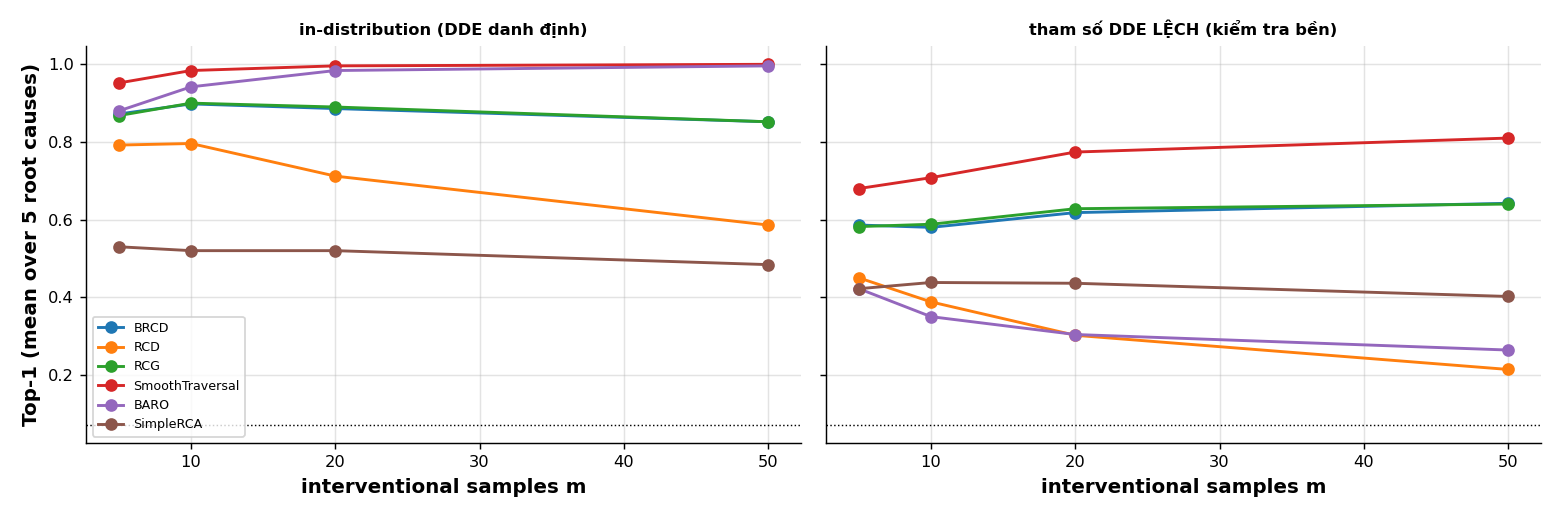
\includegraphics[width=0.95\linewidth]{figures/rca_causal.png}
\caption{Top-1 accuracy versus $m$ in the shared-generator and shifted settings (dotted line: chance).}\label{fig:causal}
\end{figure}
\paragraph{Generator shift.} With a shared generator, Smooth Traversal and BARO approach 1.0 as $m$ grows, BRCD and RCG reach 0.85--0.90, RCD declines with $m$, and SimpleRCA stays near 0.5. Under shifted parameters all methods drop and the ordering changes: BARO falls from 0.94 to 0.35 at $m{=}10$, BRCD and RCG improve slowly with $m$, and Smooth Traversal remains best at 0.71 (top-3: 0.98 Smooth Traversal, 0.93 BARO, 0.89 BRCD).
\paragraph{Graph and node ablation.} Replacing the physical graph by random edges of equal out-degree or by an empty graph changes no algorithm beyond the seed spread (BRCD $0.92\pm0.01$, $0.92\pm0.02$, $0.92\pm0.00$ shared; $0.60\pm0.05$, $0.60\pm0.05$, $0.58\pm0.06$ shifted). Every root-cause node is a graph root, so the conditional models cannot add information about it and the methods act as marginal shift detectors on the node estimates. Replacing the supervised soft sensors by label-free spectral summaries reduces accuracy to $0.07$--$0.29$ (shared) and $0.07$--$0.37$ (shifted); the simplest method reaches exactly $0.20$, consistent with only the controller-measured speed node remaining informative (not tested directly). Under shift, a threefold larger fault gain lowers accuracy (BRCD $0.60\to0.27$, Smooth Traversal $0.71\to0.28$) because soft sensors trained on nominal parameters mis-estimate larger, distorted effects.
\begin{table}[t]\centering\footnotesize
\caption{Ablation at $m{=}10$: top-1 accuracy (mean $\pm$ s.d.\ over 3 seeds) for node construction, graph and fault gain; chance $=0.07$.}\label{tab:ablation}
\begin{tabular}{p{5.6cm}cccccc}
\toprule
Variant & BRCD & RCD & RCG & Smooth & BARO & Simple \\
\midrule
\multicolumn{7}{l}{\textit{Same generator}} \\
\quad Supervised nodes, physics graph (main) & 0.92\,$\pm$\,0.01 & 0.81\,$\pm$\,0.03 & 0.92\,$\pm$\,0.01 & 0.99\,$\pm$\,0.00 & 0.91\,$\pm$\,0.07 & 0.54\,$\pm$\,0.00 \\
\quad Supervised nodes, shuffled graph & 0.92\,$\pm$\,0.02 & 0.81\,$\pm$\,0.03 & 0.92\,$\pm$\,0.01 & 0.99\,$\pm$\,0.00 & 0.91\,$\pm$\,0.07 & 0.54\,$\pm$\,0.00 \\
\quad Supervised nodes, no edges & 0.92\,$\pm$\,0.00 & 0.81\,$\pm$\,0.02 & 0.92\,$\pm$\,0.00 & 0.99\,$\pm$\,0.00 & 0.91\,$\pm$\,0.07 & 0.54\,$\pm$\,0.00 \\
\quad Label-free nodes, physics graph & 0.09\,$\pm$\,0.01 & 0.10\,$\pm$\,0.04 & 0.07\,$\pm$\,0.01 & 0.29\,$\pm$\,0.08 & 0.29\,$\pm$\,0.08 & 0.20\,$\pm$\,0.00 \\
\quad Supervised, physics graph, gain $\times0.3$ & 0.85\,$\pm$\,0.02 & 0.78\,$\pm$\,0.04 & 0.85\,$\pm$\,0.02 & 0.88\,$\pm$\,0.05 & 0.65\,$\pm$\,0.18 & 0.51\,$\pm$\,0.01 \\
\quad Supervised, physics graph, gain $\times3$ & 0.85\,$\pm$\,0.02 & 0.76\,$\pm$\,0.05 & 0.84\,$\pm$\,0.02 & 0.99\,$\pm$\,0.01 & 0.97\,$\pm$\,0.01 & 0.53\,$\pm$\,0.04 \\
\midrule
\multicolumn{7}{l}{\textit{Shifted generator parameters}} \\
\quad Supervised nodes, physics graph (main) & 0.60\,$\pm$\,0.05 & 0.43\,$\pm$\,0.05 & 0.60\,$\pm$\,0.07 & 0.71\,$\pm$\,0.07 & 0.39\,$\pm$\,0.05 & 0.45\,$\pm$\,0.01 \\
\quad Supervised nodes, shuffled graph & 0.60\,$\pm$\,0.05 & 0.42\,$\pm$\,0.05 & 0.59\,$\pm$\,0.06 & 0.71\,$\pm$\,0.07 & 0.40\,$\pm$\,0.05 & 0.45\,$\pm$\,0.01 \\
\quad Supervised nodes, no edges & 0.58\,$\pm$\,0.06 & 0.42\,$\pm$\,0.05 & 0.58\,$\pm$\,0.06 & 0.70\,$\pm$\,0.06 & 0.39\,$\pm$\,0.06 & 0.45\,$\pm$\,0.01 \\
\quad Label-free nodes, physics graph & 0.09\,$\pm$\,0.01 & 0.14\,$\pm$\,0.04 & 0.07\,$\pm$\,0.01 & 0.27\,$\pm$\,0.03 & 0.37\,$\pm$\,0.02 & 0.20\,$\pm$\,0.00 \\
\quad Supervised, physics graph, gain $\times0.3$ & 0.54\,$\pm$\,0.03 & 0.45\,$\pm$\,0.05 & 0.53\,$\pm$\,0.03 & 0.59\,$\pm$\,0.03 & 0.48\,$\pm$\,0.02 & 0.42\,$\pm$\,0.02 \\
\quad Supervised, physics graph, gain $\times3$ & 0.27\,$\pm$\,0.07 & 0.22\,$\pm$\,0.01 & 0.26\,$\pm$\,0.07 & 0.28\,$\pm$\,0.09 & 0.22\,$\pm$\,0.01 & 0.32\,$\pm$\,0.07 \\
\bottomrule
\end{tabular}

\end{table}
\paragraph{Reading.} The benchmark measures supervised estimation of the root-cause nodes and its sensitivity to generator mismatch, not causal reasoning.

\subsection{How far is the simulated healthy baseline from real data?}\label{sec:healthy}
We train the baseline on a subset of cuts and test on held-out cuts with a random-forest classifier two-sample test (balanced accuracy, folds by cut; 0.5 means indistinguishable). Table~\ref{tab:c2st} shows that all variants remain far from 0.5 ($0.82\pm0.04$ for the final model) and that kernel-regression and hierarchical variants differ within split spread. Feature means match (log acceleration $-1.37$ simulated, $-1.38$ real) but dispersion and joint dependence on conditions do not. We could not measure a floor because no cutting condition is repeated. An earlier version used plain accuracy with five synthetic windows per real one (chance 0.83); those numbers are discarded.
\begin{table}[t]\centering\small
\caption{Classifier two-sample test, real versus simulated healthy windows on held-out cuts; mean $\pm$ s.d.\ over random stratified splits.}\label{tab:c2st}
\begin{tabular}{llc}
\toprule
Mean model & Variation model & C2ST balanced accuracy $\downarrow$ \\
\midrule
Linear & mean only & 0.946 $\pm$ 0.025 \\
Linear & + between/within-cut variation & 0.853 $\pm$ 0.022 \\
Kernel ridge & mean only & 0.864 $\pm$ 0.022 \\
Kernel ridge & + between/within-cut variation (final) & \cellcolor{gray!20}\textbf{0.820 $\pm$ 0.036} \\
\bottomrule
\end{tabular}

\end{table}

\subsection{Negative result: direct calibration of the delay model}\label{sec:neg}
Fitting 15 physical and sensor parameters to real windows with CMA-ES (MMD, later group means over conditions) plateaued at a loss near 3 (squared errors in real standard deviations) and did not converge in 35--40 generations; we stopped by a pre-set rule. Earlier low-MMD fits had wrong dependence on conditions: real microphone level correlates with spindle speed at $+0.85$, the simulation gave $0.00$; simulated acceleration depended on radial depth ($0.69$), the real one did not ($0.06$). A window-length mismatch (4~s real versus 0.18~s simulated) had inflated simulated variance threefold. The data do not constrain the delay model's absolute levels, hence the use of fault \emph{differences}.

\subsection{Does any simulated fault reproduce a real defective tool?}\label{sec:real}
\paragraph{Protocol.} We compare the intentionally defective tool D$^*$ (12 cuts, 36 windows) with the healthy tool of the same type (64 cuts, 192 windows). Conditions differ, so we fit ridge models of each sensor node on the conditions with healthy cuts only (out-of-sample over cuts), express defective windows as residuals in healthy standard deviations, and bootstrap cuts for 95\% intervals (Table~\ref{tab:realshift}).
\begin{table}[t]\centering\footnotesize
\caption{Shift of each sensor node in healthy standard deviations: real defective tool D$^*$ (95\% bootstrap intervals over cuts) versus five simulated faults.}\label{tab:realshift}
\begin{tabular}{lcccccc}
\toprule
& Real tool D$^*$ & \multicolumn{5}{c}{Simulated fault} \\
\cmidrule(lr){3-7}
Sensor node [s.d.] & [95\% CI] & Stiff. & Damp. & Wear & Depth & RPM \\
\midrule
log acc.\ rms & +1.9 [+1.4, +2.5] & \cellcolor{red!18}+2.9 & \cellcolor{red!18}+2.9 & +1.9 & \cellcolor{red!18}+2.9 & \cellcolor{red!18}+3.0 \\
mic.\ level & \cellcolor{red!18}+3.6 [+3.2, +4.1] & \cellcolor{red!18}+2.3 & \cellcolor{red!18}+2.4 & +1.4 & \cellcolor{red!18}+2.3 & \cellcolor{red!18}+2.4 \\
non-sync.\ index (acc) & \cellcolor{blue!15}-3.7 [-4.3, -3.1] & -0.0 & -0.3 & -0.3 & -0.2 & +0.3 \\
non-sync.\ index (mic) & -1.2 [-1.5, -0.9] & +0.1 & -0.2 & -0.2 & -0.2 & +0.5 \\
acc.\ 50--600\,Hz & \cellcolor{red!18}+3.9 [+3.5, +4.2] & -0.0 & +0.0 & -0.0 & -0.0 & +0.0 \\
acc.\ 1--3.2\,kHz & \cellcolor{red!18}+6.3 [+5.6, +7.1] & +1.8 & +1.2 & +1.0 & +1.3 & +1.5 \\
acc.\ $>$3.2\,kHz & +1.9 [+1.4, +2.3] & +1.5 & +1.3 & +1.5 & \cellcolor{red!18}+2.1 & \cellcolor{red!18}+2.1 \\
mic.\ 50--600\,Hz & \cellcolor{red!18}+4.0 [+3.3, +4.7] & -0.0 & +0.0 & +0.0 & -0.0 & +0.1 \\
mic.\ $>$3.2\,kHz & +1.8 [+1.2, +2.3] & +0.2 & +0.2 & +0.1 & +0.3 & +0.3 \\
\midrule
Cosine with real shift & -- & 0.62 & 0.60 & 0.62 & 0.59 & 0.55 \\
\bottomrule
\end{tabular}

\end{table}
\paragraph{Result.} The real tool raises all levels, most at low frequency ($+3.9$ and $+4.0$ for the 50--600~Hz accelerometer and microphone bands) and in the 1--3.2~kHz accelerometer band ($+6.3$), and lowers both non-synchronous indices ($-3.7$, $-1.2$), i.e.\ the spectrum becomes more tonal. No simulated fault shifts low frequencies (all within $\pm0.1$) or the non-synchronous indices beyond $-0.3$ to $+0.5$. The cosine similarity to the five simulated shifts is $0.55$--$0.62$ and driven by the common ``louder'' direction.
\paragraph{Tested hypothesis: chipped flute.} We added effective runout of 10--80~$\mu$m (a once-per-revolution term) and tried fault gains of $1\times$, $10\times$, $100\times$. The cosine similarity stays at $0.48$--$0.54$, again dominated by overall level; non-synchronous indices move in the wrong direction ($+0.1$ to $+0.9$ versus $-3.7$ and $-1.2$), the low bands barely change (microphone low band $\le+0.9$ versus $+4.0$), and the high accelerometer band grows far too much ($+1$ to $+38$ versus $+1.9$ with added gain). A once-per-revolution runout therefore does not reproduce the signature either. Per-tooth force asymmetry and nonlinear edge or friction effects remain untested.
\paragraph{Scope.} The tools differ (12.7~mm four-flute steel versus simulated 6.35~mm two-flute aluminium), so only direction and sign in standardised units are compared.

\subsection{Sensitivity to the assumed fault strength}\label{sec:sweep}
Scaling the fault gains by $0.3$ and $3$ changes the best simulated classifier's accuracy from $0.698$ to $0.943$ (Table~\ref{tab:sweep}); six-class accuracy within the simulator (Table~\ref{tab:cls}, 16 held-out cuts) is therefore only interpretable together with this curve. Applied to real windows, 91--97\% of normal windows are classified normal by tree and neighbour models but only 51\% and 57\% by logistic regression and Naive Bayes, and 61, 64 and 72 of 75 real abnormal windows are assigned to tool wear by QDA, random forest and gradient boosting; with no ground truth for abnormal windows we read this as mapping any broadband increase to wear.
\begin{table}[t]\centering\small
\caption{Top-1 accuracy of classifiers on simulated data versus fault gain relative to the calibrated value.}\label{tab:sweep}
\begin{tabular}{lccc}
\toprule
Classifier & gain $\times0.3$ $\uparrow$ & $\times1$ (calibrated) $\uparrow$ & $\times3$ $\uparrow$ \\
\midrule
Gradient boosting & \cellcolor{gray!20}\textbf{0.698} & \cellcolor{gray!20}\textbf{0.882} & \cellcolor{gray!20}\textbf{0.943} \\
Random forest & 0.674 & 0.855 & 0.922 \\
QDA (Bayes) & 0.545 & 0.769 & 0.847 \\
Logistic regression & 0.535 & 0.729 & 0.834 \\
\bottomrule
\end{tabular}

\end{table}
\begin{table}[t]\centering\small
\caption{Six-class classification on simulated data, 16 held-out cuts (chance $0.167$).}\label{tab:cls}
\begin{tabular}{lcccc}
\toprule
Classifier & Top-1 $\uparrow$ & Top-3 $\uparrow$ & Macro-F1 $\uparrow$ & AUROC$_{\text{fault vs.\ normal}}$ $\uparrow$ \\
\midrule
Gradient boosting & \cellcolor{gray!20}\textbf{0.886} & \cellcolor{gray!20}\textbf{0.990} & \cellcolor{gray!20}\textbf{0.885} & \cellcolor{gray!20}\textbf{1.000} \\
Random forest & 0.870 & \cellcolor{gray!20}\textbf{0.990} & 0.868 & 0.998 \\
MLP & 0.807 & 0.987 & 0.804 & 0.994 \\
QDA (Bayes) & 0.787 & 0.978 & 0.779 & 0.992 \\
Logistic regression & 0.726 & 0.966 & 0.722 & 0.990 \\
kNN & 0.722 & 0.922 & 0.717 & 0.983 \\
Gaussian Naive Bayes & 0.579 & 0.912 & 0.554 & 0.961 \\
\bottomrule
\end{tabular}

\end{table}

\subsection{When does simulation help on real data? Cross-machine wear}\label{sec:wear}
\paragraph{Setup.} LUH has three machines and three tools per machine with measured flank wear (VB). The target is wear $\ge100~\mu$m (AUROC; chance 0.5; 406 runs, 26\% positive). Features are force-based (means, standard deviations, kurtosis, band powers of $x$, $y$ and the resultant).
\paragraph{Cross-machine transfer with real labels.} Table~\ref{tab:luh} shows that wear detection is easy: AUROC is already $0.94$--$0.96$ for a new tool on the same machine and $0.92$--$0.99$ for an unseen machine. Normalising features by each machine's healthy baseline did not raise AUROC (gradient boosting, unseen machine: $0.990$ raw, $0.955$ machine-relative, $0.986$ tool-relative) and increased the wear-estimation error (MAE of VB $9.2$, $17.7$, $11.1~\mu$m).
\begin{table}[t]\centering\small
\caption{Wear detection (AUROC, gradient boosting) and VB error on LUH. E1: new tool, same machine; E2: unseen machine, trained on two; E3: unseen machine, trained on one.}\label{tab:luh}
\begin{tabular}{lcccccc}\toprule
 & \multicolumn{3}{c}{AUROC $\uparrow$} & \multicolumn{3}{c}{MAE VB [$\mu$m] $\downarrow$}\\\cmidrule(lr){2-4}\cmidrule(lr){5-7}
Features & E1 & E2 & E3 & E1 & E2 & E3\\\midrule
Raw & 0.964 & \best{0.990} & \best{0.982} & 9.2 & 9.2 & 11.3\\
Machine-relative & 0.964 & 0.955 & 0.942 & 9.2 & 17.7 & 28.4\\
Tool-relative & 0.937 & 0.986 & 0.915 & 12.4 & 11.1 & 10.9\\\bottomrule
\end{tabular}
\end{table}
\paragraph{Baselines for unseen machines.} Table~\ref{tab:luhbase} adds a one-feature rule (mean resultant force, higher means worn, no labels needed), CORAL and DANN, which use unlabelled target-machine features (transductive), with 10 seeds. The one-feature rule reaches AUROC $0.996$ and $0.993$ on machines 1 and 2 with raw features but $0.46$ on machine 3, so force scale differs across machines; gradient boosting with raw features is $\ge0.976$ on all three. Domain adaptation does not improve on gradient boosting (raw features: DANN $0.996/0.997/0.974$, CORAL+LR $0.992/0.995/0.886$), and tool-relative features make DANN unstable (machine 1: $0.79\pm0.13$). Bootstrap intervals are over runs and understate uncertainty because runs of one tool are correlated; gradient boosting and logistic regression are deterministic, so their seed spread is zero.
\begin{table}[t]\centering\small
\caption{Leave-one-machine-out wear detection, AUROC $\uparrow$ (mean over 10 seeds) on target machines 1/2/3. Raw features; other feature sets in \texttt{output/luh\_baselines.json}.}\label{tab:luhbase}
\begin{tabular}{lccc}\toprule
Method & M1 & M2 & M3\\\midrule
One-feature RMS rule (no labels) & 0.996 & 0.993 & 0.462\\
Gradient boosting & 0.995 & \best{0.999} & \best{0.976}\\
Logistic regression & 0.996 & 0.995 & 0.943\\
CORAL + LR (unlabelled target) & 0.992 & 0.995 & 0.886\\
DANN (unlabelled target) & \best{0.996} & 0.997 & 0.974\\
Simulation only, no real labels & 0.887 & 0.807 & 0.571\\\bottomrule
\end{tabular}
\end{table}
\paragraph{Simulation without real labels.} A classifier trained only on simulated wear and applied to the three target machines reaches AUROC $0.887$, $0.807$ and $0.571$ (machines 1, 2, 3) using sign-invariant features. The first attempt with signed mean force was below chance (AUROC $0.55$, $0.26$, $0.10$) because of an axis sign convention; changing to absolute mean force was decided after seeing this result, though with a physical argument, so the numbers should be read as exploratory.
\paragraph{Fine-tuning.} Fine-tuning from the simulated solution with $k$ real samples was not better than training from scratch at any $k$ (AUROC $0.83$--$0.89$ versus $0.85$--$0.89$ at $k{=}2$; $0.97$--$0.99$ versus $0.99$ at $k{=}32$). On this easy task a few real labels already suffice.
\paragraph{Earlier wear thresholds.} Because a detection of heavy wear may be too easy, we repeated the label-free comparison at wear thresholds VB $\ge60$ and $\ge40~\mu$m (the thresholds were fixed before running; all three are reported). The comparator is the one-feature resultant-force rule computed on the same tool-relative $x,y$ features, which needs no labels either (Table~\ref{tab:thr}). Averaged over machines, the simulation-only model is higher than the rule at every threshold ($0.76$ vs.\ $0.74$, $0.83$ vs.\ $0.74$, $0.83$ vs.\ $0.78$), but the gain comes from machine~3, where the rule is below chance ($0.42$, $0.40$ and $0.43$) and simulation reaches $0.57$--$0.78$; on machines 1 and 2 the rule is as good as or better than simulation in five of six cases (machine 1 at $60~\mu$m is tied). Fine-tuning from the simulated solution was again no better than learning from scratch at any $k$ (for example at $k{=}2$ and $\lambda{=}1$: $0.83$ vs.\ $0.85$ at $100~\mu$m, $0.90$ vs.\ $0.94$ at $60~\mu$m, $0.87$ vs.\ $0.97$ at $40~\mu$m). The evidence for a label-free benefit of simulation is therefore limited to one of three machines, with the sign of the one-feature rule on that machine unexplained; a benefit of simulation would have to be shown on harder, multi-cause tasks that we cannot test yet.
\begin{table}[t]\centering\small
\caption{Label-free wear detection on unseen machines, AUROC $\uparrow$ (M1/M2/M3 and mean), by wear threshold. Rule: mean resultant force on tool-relative $x,y$ features.}\label{tab:thr}
\begin{tabular}{lcccc}\toprule
Threshold & Method & M1 / M2 / M3 & Mean\\\midrule
\multirow{2}{*}{VB $\ge100~\mu$m} & Rule & 0.853 / 0.936 / 0.433 & 0.741\\
 & Simulation & 0.887 / 0.807 / 0.571 & \best{0.755}\\\midrule
\multirow{2}{*}{VB $\ge60~\mu$m} & Rule & 0.927 / 0.870 / 0.415 & 0.737\\
 & Simulation & 0.925 / 0.809 / 0.759 & \best{0.831}\\\midrule
\multirow{2}{*}{VB $\ge40~\mu$m} & Rule & 0.994 / 0.941 / 0.398 & 0.778\\
 & Simulation & 0.827 / 0.893 / 0.782 & \best{0.834}\\\bottomrule
\end{tabular}
\end{table}

%% ---------------------------------------------------------------------------------------------
\paragraph{Does real-data transfer degrade when the target dynamics are far from the training machines?} Without measured transfer functions for LUH we used a proxy: the mean 21-band force spectrum of the three least-worn runs of each tool. For each of the nine target tools we trained on the tools of the other machines (all six, the three nearest, the three farthest by the proxy). With gradient boosting and raw features at VB $\ge100~\mu$m, AUROC was $0.993$, $0.984$ and $0.976$ for all, nearest and farthest training tools; the Spearman correlation between proxy distance and AUROC was $-0.16$ ($p=0.67$) at VB $\ge100~\mu$m and $-0.34$ ($p=0.36$) at $60~\mu$m. Only logistic regression on tool-relative features at $60~\mu$m showed a trend ($\rho=-0.62$, $p=0.08$; lowest AUROC $0.25$). With nine targets, a weak proxy and an unknown range of dynamics, this is absence of evidence, not evidence of absence: on these data real-data transfer is sufficient, and the question whether simulation is needed to reach dynamics outside the training range remains open.

\section{Limitations and Next Steps}\label{sec:limits}
\paragraph{Scope limits.} Results are for one tool and material (MSM subset), one defective-tool comparison on a different tool, and force-only wear data (LUH). We have no real multi-cause data and therefore no validation of root-cause ranking on real cuts.
\paragraph{Open technical limits.} (i) The healthy baseline remains distinguishable from real data (balanced accuracy $0.82$--$0.95$ over the four variants); (ii) neither standard fault models nor a chipped-flute runout reproduces the defective-tool signature; (iii) the MSM microphone and accelerometer show a machine line near 1.5~kHz that contaminates the 1--3~kHz features; (iv) main causal tables use one split and seed, and only the ablation reports three seeds; (v) fault severity ranges, gains, nominal physical parameters and the causal graph are assumptions; (vi) FRF import is tested only on synthetic transfer functions.
\paragraph{Planned evaluation on real multi-cause data.} The full collection and evaluation protocol is in \texttt{paper/DATA\_PROTOCOL.md}; the central test is leave-one-configuration-out over machine--tool--overhang configurations with measured FRFs, comparing real data only, FRF-anchored simulation only and their combination. We will collect cuts with designed causes (clamp stiffness, overhang, wear, depth or speed outside the stable range, imbalance, chipped flute) on at least two machines with hammer-test FRFs and force-coefficient calibration cuts, and evaluate by leave-one-machine-out and leave-one-configuration-out with: simulation only ($k{=}0$), simulation plus $k$ real samples, real only; top-1/top-3, macro-F1, calibration error and coverage--accuracy for an abstain option. Baselines: standard classifiers, domain-adversarial transfer \citep{wang2020datwear}, meta domain generalisation \citep{li2023metadg}, RMS and spectral-rule thresholds, and FRF-based stability checks. Decision gates: if the simulator with measured FRFs does not reproduce the measured stability boundary within an agreed tolerance, fix the model before collecting more; if no benefit at small $k$ appears, position the contribution as zero-shot ($k{=}0$), dataset and gap analysis.

\section{Conclusion}
We asked how far simulation can take root cause diagnosis in milling and measured it against real data in three places.
Simulated causal-RCA accuracy depends on how diagnostic nodes are built and falls from 0.80--0.98 to 0.35--0.71 under moderate generator mismatch, while the causal graph has no effect; the simulated healthy baseline and the signature of a real defective tool remain different from real data; and on a public wear dataset simulation-only transfer is below a one-feature rule on two machines and brings no fine-tuning benefit, because the task is too easy to show one.
Simulation is necessary in principle for causes without real labels, but its value was not demonstrated on any real task we could test. These results define where simulation cannot yet be trusted and give a protocol to test it on real multi-cause data, which is the main limitation and the next step.

\paragraph{Code and data.} Code: project repository (branch \texttt{cutting-sim-experiments}); data: MSM \citep{kim2026msm} (CC BY 4.0), LUH \citep{denkena2023luh}. \todo{release instructions}

\bibliographystyle{plainnat}
\bibliography{refs}

\appendix
\section{Parameter provenance}\label{app:registry}
\begin{table}[h]\centering\small
\caption{Every simulator parameter, its tier (fixed / range / learned / assumed) and verification status.}
\begin{tabular}{p{5.2cm}p{1.8cm}p{6.5cm}}
\toprule
Parameter & Tier & Verification \\
\midrule
tool diameter, flutes, flute length, overall length & FIXED & verified (read from catalog table p.5) \\
helix angle $\beta$ & FIXED & medium: from series feature list (p.3); not stated per part number \\
tool substrate/coating & FIXED & medium \\
N, ae, feed F, direction & FIXED & verified (N and F equal mtc Spindle\_Speed/Feed\_Rate, ratio 1.000) \\
axial depth ap = engaged depth & FIXED & assumption (not measured) \\
workpiece AA 6061; wet cutting (coolant flood) & FIXED & verified (stated in paper) \\
sampling: accelerometer 51.2 kHz, audio 48 kHz & FIXED & verified (stated in paper) \\
analysis window 0.3 s & FIXED & design choice \\
model structure: regenerative DDE, shear+edge force, ZOA lobes & FIXED & model structure \\
\midrule
Kt, Kr, Kte, Kre (AA 6061, this tool, wet) & LEARNED & NO usable source (rejected: steel-like values; dry-cutting AA6061 value unverified) \\
tool-tip FRF: fn\_x, fn\_y, $\zeta$, modal stiffness k & LEARNED & NO source for this tool/holder/stick-out (Altintas Ex.2 FRF rejected: different machine and tool) \\
spindle imbalance U & LEARNED & NO source (rotor mass, balance grade unknown) \\
sensor gains, noise floors, rpm-dependence & LEARNED & NO source (sensors uncalibrated: mic dBFS, accelerometer mm/s\^{}2) \\
runout; between-cut variability $\sigma$ (Kt, runout, roughness) & LEARNED & NO source \\
\midrule
chip-thickness cap 0.3 mm; roughness noise base 0.02 $\mu$m & ASSUMED & own assumption \\
\bottomrule
\end{tabular}

\end{table}

\section{Methodological pitfalls found along the way}
\begin{enumerate}
\item Plain accuracy of a classifier two-sample test with unequal sizes has a chance level above 0.5; use balanced accuracy.
\item Real and simulated features must use windows of identical length; a 20-fold mismatch inflated variance threefold.
\item Out-of-sample residuals are needed to estimate between-cut variation when the regression can interpolate each cut.
\item Distribution matching alone did not identify the fault gain; effect-size matching was used.
\item Nodes trained on the generator's labels make a causal benchmark circular.
\item Force-axis sign conventions differ between machines; a signed mean force put zero-shot transfer below chance.
\end{enumerate}
\end{document}
